\begin{frame}{Kiến trúc Dịch vụ Thanh toán (Payment Service)}
\begin{figure}[H]
\centering
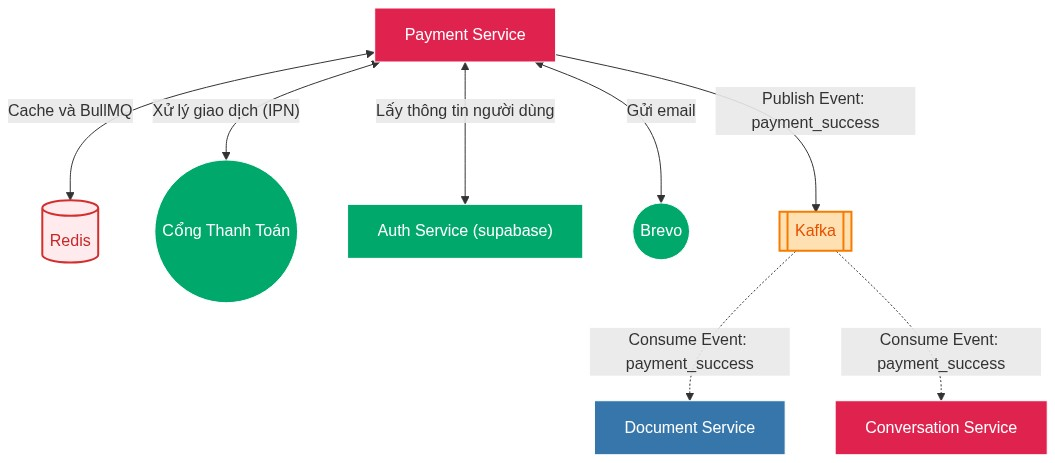
\includegraphics[height=0.7\textheight,width=0.9\textwidth,keepaspectratio]{pictures/payment-kafka-event.png}
\caption{Sơ đồ tổng quan dịch vụ thanh toán}
\end{figure}

\note{
Dịch vụ thanh toán (Payment Service) chịu trách nhiệm quản lý thông tin các gói dịch vụ (Plans), quản lý thuê bao người dùng (Subscriptions) và tích hợp với cổng thanh toán ngoại vi.
Khi người dùng thực hiện thanh toán thành công, dịch vụ này sẽ phát đi sự kiện \texttt{payment\_success} vào hệ thống truyền tin nhắn Kafka để các dịch vụ khác như Chatbot và Document cập nhật quyền VIP cho người dùng.
}
\end{frame}
